\documentclass[11pt]{aghdpl}
% \documentclass[en,11pt]{aghdpl}  % praca w języku angielskim

% Lista wszystkich języków stanowiących języki pozycji bibliograficznych użytych w pracy.
% (Zgodnie z zasadami tworzenia bibliografii każda pozycja powinna zostać utworzona zgodnie z zasadami języka, w którym dana publikacja została napisana.)
\usepackage[english,polish]{babel}

% Użyj polskiego łamania wyrazów (zamiast domyślnego angielskiego).
\usepackage{polski}

\usepackage[utf8]{inputenc}

% dodatkowe pakiety

\usepackage{mathtools}
\usepackage{amsfonts}
\usepackage{amsmath}
\usepackage{amsthm}


% --- < bibliografia > ---

\usepackage[
backend=biber,
style=numeric,
sorting=none,
%
% Zastosuj styl wpisu bibliograficznego właściwy językowi publikacji.
language=autobib,
autolang=other,
% Zapisuj datę dostępu do strony WWW w formacie RRRR-MM-DD.
urldate=iso8601,
% Nie dodawaj numerów stron, na których występuje cytowanie.
backref=false,
% Podawaj ISBN.
isbn=true,
% Nie podawaj URL-i, o ile nie jest to konieczne.
url=false,
%
% Ustawienia związane z polskimi normami dla bibliografii.
maxbibnames=3,
]{biblatex}

\usepackage{csquotes}
% Ponieważ `csquotes` nie posiada polskiego stylu, można skorzystać z mocno zbliżonego stylu chorwackiego.
\DeclareQuoteAlias{croatian}{polish}

\addbibresource{bibliografia.bib}

% Nie wyświetlaj wybranych pól.
%\AtEveryBibitem{\clearfield{note}}


% ------------------------
% --- < listingi > ---

% Użyj czcionki kroju Courier.
\usepackage{courier}

\usepackage{listings}
\lstloadlanguages{TeX}

\lstset{
	literate={ą}{{\k{a}}}1
           {ć}{{\'c}}1
           {ę}{{\k{e}}}1
           {ó}{{\'o}}1
           {ń}{{\'n}}1
           {ł}{{\l{}}}1
           {ś}{{\'s}}1
           {ź}{{\'z}}1
           {ż}{{\.z}}1
           {Ą}{{\k{A}}}1
           {Ć}{{\'C}}1
           {Ę}{{\k{E}}}1
           {Ó}{{\'O}}1
           {Ń}{{\'N}}1
           {Ł}{{\L{}}}1
           {Ś}{{\'S}}1
           {Ź}{{\'Z}}1
           {Ż}{{\.Z}}1,
	basicstyle=\footnotesize\ttfamily,
}

% ------------------------

\AtBeginDocument{
	\renewcommand{\tablename}{Tabela}
	\renewcommand{\figurename}{Rys.}
}

% ------------------------
% --- < tabele > ---

\usepackage{array}
\usepackage{tabularx}
\usepackage{multirow}
\usepackage{booktabs}
\usepackage{makecell}
\usepackage[flushleft]{threeparttable}

% defines the X column to use m (\parbox[c]) instead of p (`parbox[t]`)
\newcolumntype{C}[1]{>{\hsize=#1\hsize\centering\arraybackslash}X}


%---------------------------------------------------------------------------

\author{Marek Ryznar}
\shortauthor{M. Ryznar}

%\titlePL{Przygotowanie bardzo długiej i pasjonującej pracy dyplomowej w~systemie~\LaTeX}
%\titleEN{Preparation of a very long and fascinating bachelor or master thesis in \LaTeX}

\titlePL{Serwis internetowy dla studentów zaimplementowany w architekturze SOA}
\titleEN{Internet service for students implememented in SOA architecture}


\shorttitlePL{} % skrócona wersja tytułu jeśli jest bardzo długi
\shorttitleEN{}

\thesistype{Praca dyplomowa inżynierska}
%\thesistype{Bahelor of Science Thesis}

\supervisor{dr inż. Mirosław Gajer}
%\supervisor{Mirosław Gajer PhD, DSc}

\degreeprogramme{Informatyka}
%\degreeprogramme{Computer Science}

\date{2015}

\department{Katedra Informatyki Stosowanej}
%\department{Department of Applied Computer Science}

\faculty{Wydział Elektrotechniki, Automatyki,\protect\\[-1mm] Informatyki i Inżynierii Biomedycznej}
%\faculty{Faculty of Electrical Engineering, Automatics, Computer Science and Biomedical Engineering}

\acknowledgements{Serdecznie dziękuję \dots tu ciąg dalszych podziękowań np. dla promotora, żony, sąsiada itp.}


\setlength{\cftsecnumwidth}{10mm}

%---------------------------------------------------------------------------
\setcounter{secnumdepth}{4}

\begin{document}

\titlepages

% Ponowne zdefiniowanie stylu `plain`, aby usunąć numer strony z pierwszej strony spisu treści i poszczególnych rozdziałów.
\fancypagestyle{plain}
{
	% Usuń nagłówek i stopkę
	\fancyhf{}
	% Usuń linie.
	\renewcommand{\headrulewidth}{0pt}
	\renewcommand{\footrulewidth}{0pt}
}

\setcounter{tocdepth}{2}
\tableofcontents
\clearpage

\chapter{Wprowadzenie}
\label{cha:wprowadzenie}

W dobie współczesnej technologii i internetu, wymiana notatek z zajęć dydaktycznych oraz przekazywanie sobie wzajemnie przez studentów informacji dotyczących odwołanych zajęć bądź też informacji o kolokwiach i egzaminach, nie stanowi problemu. Najbardziej znanym sposobem na wymianę plików jest wysyłanie za pomocą wiadomości email. Często niestety bywa tak, że załączone materiały przekraczają dopuszczalny rozmiar załącznika, wtedy z pomocą przychodzą dyski internetowe, które pozwalają na przechowywanie większych plików. Najbardziej znane wśród studentów to google drive, dropbox i One drive.

Wszystkie wymienione wyżej rozwiązania są często stosowane przez studentów, aczkolwiek trudno znaleść odpowiedni serwis dedykowany bezpośrednio dla nich. Celem tej pracy jest implementacja serwisu internetowego pomagającego w zarządzaniu materiałami dydaktycznymi z zajęć. Głównym przeznaczeniem tworzonego portalu jest dodawanie plików oraz udostępnianie ich innym użytkownikom. Dodatkową planowaną  funkcjonalnością, która może pomóc studentowi w organizacji roku akademickiego jest przeznaczony dla niego kalendarz, w którym użytkownik mógłby zapisywać wszystkie ważne wydarzenia takie jak kolokwia lub egzaminy. Kolejną funkcją systemu, która ma na celu ułatwienie studentowi zarządzania kontem serwisu jest strona powiadomień na której znajdować się będą przypomnienia o zbliżających się wydarzeniach, informacje o udostępnionych dla niego plikach oraz informacje dotyczące uczelni.

Niniejsza praca opisuje proces powstawania przedstawionego serwisu. W pierwszym rozdziale czytelnik zostanie zaznajomiony z najważniejszymi pojęciami dotyczącymi opisywanego projektu. W kolejnym rozdziale znajduje się koncepcja systemu przedstawiona za pomocą dokładnie opisanych (słownie oraz za pomocą diagramów czynności oraz przypadków użycia) zaplanowanych funkcji systemu. W czwartym rozdziale za pomocą modelu bazy danych oraz modelu klas przedstawiony jest projekt systemu. Na samym końcu opisane są najważniejsze szczegóły implementacyjne projektu.
\chapter{Podstawy teoretyczne}
\label{cha:podstawyTeoretyczne}
Rozdział ten przedstawia podstawy teoretyczne projektu. W pierwszym porozdziale znajduje się krótkie wprowadzenie do architektóry SOA, na której oparty jest serwis. W następnym opisany jest język implementacji. Trzeci podrozdział prezentuje formę przechowywania danych w serwisie. Ostatni punkt zaznajamia nas z przenaczeniem serwerów aplikacyjnych i konkretnym zastosowaniu w implementowanym projekcie.

%---------------------------------------------------------------------------

\section{SOA}
\label{sec:soa}

Rozwinięciem skrótu SOA jest \textit{Service Oriented Architecture} czyli architektura zorientowana na usługi. Według książki \textit{SOA Design Principles for Dummies} SOA składa się z trzech podstawowych aspektów:
\begin{itemize}
	\item \textbf{Usługa} - czyli powtarzalne zadanie biznesowe np. Dodawanie plików na serwer lub tworzenie nowego konta.
	\item \textbf{Orientacja na usługi} - Sposób postrzegania produktu jako zbiór usług połączonych w całość.
	\item \textbf{SOA} - Podejście architektoniczne bazujące na zasadach orientacji na usługi.
\end{itemize}
Architektura zorientowana na usługi posiada następujące właściwości:
\begin{itemize}
	\item \textbf{Luźne powiązanie usług}
	\item \textbf{Abstrakcyjne usługi}
	\item \textbf{Autonomiczność usług}
	\item \textbf{Możliwość wielokrotnego użycia usług}
	\item \textbf{Bezstanowość usług}
	\item \textbf{Dzielenie usług na komponenty}
\end{itemize}
\cite{SOA13}
SOA jest architekturą wspierającą modularność więc produkty pisane w tej architekturze łatwo jest rozwijać poprzez dodawanie nowych usług. \newline

\section{Java}
\label{sec:java}

Język programowania Java został stworzony na początku lat dziewięćdziesiątych przez grupę inżynierów z firmy Sun zwaną "Green Team". Ideą tworzonego języka była praca w rozwijającym się środowisku internetu \cite{Java01}. Java została uformowana na podstawie języka C++ przy czym wymusza ona programowanie obiektowe. Jest jednym z najbardziej popularnych języków programowania i każdy kto miał jakąkolwiek styczność z programowaniem przynajmniej o nim słyszał (Tutaj mam nadzieje, że Paulinka mi zrefaktorujesz to zdanie). 

Java dzięki swojej platformie programistycznej Java EE (Java Enterprise Edition) pozwala pisać multi platformowe, wielowarstwowe niezawodne i bezpieczne aplikacje sieciowe. Dzięki wielu darmowo udostępnianym bibliotekom i frameworkom wielu programistów decyduje się na wybranie tej właśnie platformy \cite{JEE01}. W swojej pracy główne frameworki platformy Java EE pomagające w tworzeniu opisywanej aplikacji to:
\begin{itemize}
	\item \textbf{JSF} - Java Server Faces, który upraszcza tworzenie internetowego interfejsu użytkownika, dzięki udostępnianym tagom, z których można korzystać tworząc strony www. Posiada także Managed Beany czyli klasy odpowiedzialne za połączenie logiki aplikacji z widokiem czyli ze stronami internetowymi.
	\item \textbf{Hibernate} - jest to biblioteka dla języka Java dostarczającą framework do realizacji warstwy dostępu do danych. Zapewnia translację danych z relacyjnej bazy danych na klasy Java i vice versa (Object/Relational Mapping). Zastępuje bezpośrednie metody dostępu do danych za pomocą wysokopoziomowych metod operujących na zmapowanych obiektach.
\end{itemize}

%---------------------------------------------------------------------------

\section{Przechowywanie danych}
\label{sec:bazadanych}
Wirtualne dane można przechowywać na wiele sposobów, najprostszym z nich jest przechowywanie danych lokalnie czyli na dysku twardym stacji roboczej, aczkolwiek w tym wypadku istnieje zagrożenie utraty tych danych w razie zepsucia się komputera. W obawie przed utratą danych użytkownicy często szukają sposobu na umieszczenie ich zapasowej kopii w internecie. Istnieje wiele sposobów na przechowywanie naszych plików w internecie:
\begin{itemize}
	\item \textbf{Dyski sieciowe} - jest to typ urządzenia przechowującego dane, które zapewnia dostęp do nich w lokalnej sieci LAN.
	\item \textbf{Dyski internetowe} - umożliwiają przechowywanie plików w "internecie", tzn. korzystają między innymi z chmur internetowych do zapisu danych. 
	\item \textbf{Bazy danych} - z tego rozwiązania korzysta się raczej w przypadku ustrukturyzowanych danych np. Informacje o użytkownikach (login użytkownika serwisu w postaci krótkiego pola tekstowego lub rok jego urodzenia w postaci liczby naturalnej). Pomimo tego niektóre bazy danych udostępniają możliwość przechowywania danych w postaci binarniej czyli bez podania ich typu co pozwala na zapisywanie danych bez wymuszonego ich typu.  
\end{itemize}

Do implementacji aplikacji użyto bazy danych. Wybór był podyktowany tym, że platforma Java EE udostępnia framework Hibernate, który pozwala na prosty dostęp do bazy danych. Wybrany system do zarządzania relacyjną bazą danych to PostgreSQL, system ten jest wolnodostępny. Do przechowywania danych o użytkownikach i ich kalendarzach wystarczą podstawowe typy danych dostępne we większości sytemów zarządzających bazą danych. Do przechowywania większych plików takich jak całe książki w dowolnym formacie służy typ danych BLOB czyli Binary Large Objects co jak sama nazwa wskazuje służy do przechowywania większych plików binarnych.
%---------------------------------------------------------------------------
\section{Serwer Aplikacyjny}
\label{sec:serweraplikacyjny}
Serwer aplikacyjny jest kontenerem webowym, który odpowiada za przechowywanie, zdalne uruchamianie i użytkowanie aplikacji Java EE. Ponadto pomaga programiście tworzyć aplikacje oraz umożliwia oddzielenie logiki biznesowej od usług dostarczanych przez dany serwer aplikacyjny np. zabezpieczenia aplikacji \cite{SA01}. Najbardziej znane serwery aplikacyjne to JBoss, IBM WebSphere, Apache Tomcat, GlassFish. Serwer używany do implementacji opisywanej aplikacji to JBoss AS 7.1.1. Serwer ten został wybrany ponieważ jest darmowy (udostępniany na licencji \textit{GNU Lesser General Public License}), ponadto implementuje pełen zestaw usług JEE. Dodatkowym argumentem przemawiającym za wyborem właśnie tego serwera była jego intergracja z Eclipse (środowiskiem programistycznym w którym wykonany został projekt) za pomocą wtyczki JBossTools co znacznie ułatwiło pracę. 

\chapter{Projekt systemu}
\label{cha:projektSystemu}
Rozdział ten w 3 podrozdziałach przedstawia koncepcję implementowanej aplikacji. W podrozdziale pierwszym opisany jest system, w drugim znajduje się specyfikacja wymagań, a w trzecim model systemu. Dokumentacja projektu została częściowo oprata na szablonie dokumentacji projektu stworzonym przez dr Piotra Szweda \cite{DOC01}.
\section{Opis systemu}
W tym podrozdziale opisany jest cel systemu, jego granice, lista możliwości systemu oraz jego użytkownicy. Ponadto za pomocą diagramów aktywności przedstawione jest działanie aplikacji.
\subsection{Cel projektu}
Celem projektu jest implementacja serwisu internetowego dedykowanego dla studentów w architekturze SOA. Głównym zadaniem serwisu ma być możliwość przechowywania plików oraz udostępnianie ich innym użytkownikom. Ponadto każdy z użytkowników będzie mógł korzystać z dedykowanego dla niego kalendarza, w którym może zapisywać ważne wydarzenia. Oprócz opisanych wcześniej funkcji użytkownik za pomocą strony powiadomień będzie mógł się dowiedzieć o nadchodzących wydarzeniach oraz o udostępnionych dla niego plikach.

\subsection{Użytkownicy}
Grupę użytkowników stanowią wszyscy korzystającyz serwisu, z wyszczególnieniem:
\begin{itemize}
	\item \textbf{Użytkownik} - Docelowym użytkownikiem serwisu jest student potrzebujący dodać lub uzyskać dostęp do pliku poprzez udostępnienie od innych użytkowników serwisu. Nie jest warunkiem koniecznym, aby użytkownik był studentem.
	\item \textbf{Administrator} - Użytkownik posiadający szystkie uprawnienia, takie jak usówanie użytkowników oraz wgląd do wszystkich plików w systemie.
\end{itemize}

\subsection{Granice systemu}
Granicą systemu dla użytkownika jak i dla administratora będzie strona internetowa aplikacji. Zawarty będzie tam dostęp do wszystkich funkconalności systemu. Administrator dodatkowo będzie miał dostęp do specjalnego panelu za pomocą którego będzie mógł zarządzać kontami wszystkich użytkowników.

Wejścia w systemie:
\begin{itemize}
	\item formularz nowego konta – użytkownik wypełnia dane: login, hasło, imie, nazwisko, adres e-mail,
	\item formularz logowania – zalogowanie się do systemu za pomocą loginu i hasła użytkownika,
	\item formularz edycji konta – zmiana danych użytkownika,
	\item formularz nowego pliku – załączonik oraz opcjonalnie tytuł i opis pliku,
	\item formularz edycji pliku - zmiana załącznika, tytułu lub opisu,
	\item formularz udostępnienia pliku - login użytkownika, któremu ma być udostępniony wybrany plik,
	\item formularz nowego wydarzenia - wybrana data, nazwa wydarzenia oraz opcjonalny opis,
	\item formularz edycji wydarzenia - nowe dane do wybranego wydarzenia,
\end{itemize}
Wyjścia w systemie:
\begin{itemize}
	\item Strona powiadomień - na tej stronie znajdować się będą informacje o udostępnionych plikach oraz o przypomnienia o nadchodzących wydarzeniach.
	\item Strona przeglądania własnych plików - użytkownik na tej stronie może przeglądać dodane przez siebie pliki,
	\item Strona przeglądania udostępnionych plików - tutaj użytkownik będzie mógł przeglądać pliki mu udostępnione,
	\item Strona kalendarza - Strona odpowiedzialna za wyświetlanie kalendarza.
\end{itemize}
\subsection{Lista możliwości}
\label{listaFun}
Lista wymagań funkcjonalnych:
\begin{itemize}
	\item Logowanie,
	\item Wylogowanie,
	\item Rejestracja,
	\item Zarządzanie kontem,
	\item Zarządzanie materiałami,
	\item Pobieranie pliku,
	\item Udostępnianie pliku,
	\item Zarządzanie kalendarzem,
	\item Otrzymywanie powiadomień,
\end{itemize}

Dodatkowe funkcje administratora:
\begin{itemize}
	\item Zarządzanie kontami użytkowników.
\end{itemize}

Na kolejnych stronach zostały przedstawione diagramy czynności typowych akcji.

	
\section{Specyfikacja i analiza wymagań}
Dzięki analizie wymagań funkcjonalnych możemy zidentyfikować oczekiwane zachowania budowanego systemu. Wymaganie funkcjonalne jest to „stwierdzenie, jakie usługi ma oferować system, jak ma reagować na określone dane wejściowe oraz jak ma się zachowywać w określonych sytuacjach. W niektórych wypadkach wymagania funkcjonalne określają, czego system nie powinien robić” \cite{DOC02}. W tym podrozdziale opisane zostaną lista wymagań wunkonalnych oraz niefunkcjonalnych oraz przedstawiony zostanie diagram przypadków użycia z dołączonymi scenariuszami.
\subsection{Wymagania oprogramowania}
Wymagania funkcjonalne zostały wypisane w podpunkcie \ref{listaFun}.
Wymagania niefunkcjonalne:
\begin{enumerate}
	\item Wymaganie organizacyjne:
		\begin{itemize}
			\item Implementacji : językiem programowania jest Java,
			\item Użyteczności : Interfejs graficzny użytkownika jest przejrzysty i łatwy do przyswojenia,
		\end{itemize}
	\item Wymagania zewnętrzne:		
		\begin{itemize}
			\item Poufności - Projekt przestrzega wymagań prawnych ustanowionych w Ustawie o Ochronie Danych Osobowych.
			\item Bezpieczeństwa : System nie pozwala użytkownikom na nieautoryzowany dostęp do bazy danych
		\end{itemize}
\end{enumerate}
\subsection{Ryzyka operacyjne}
Ryzykiem w implementowanym systemie może być niedostateczne zabezpieczenie bazy danych lub pojawienie się nieobsłużonych błędów.
//TODO: Poszukać i dodać tu jeszcze cos
\subsection{Przypadki użycia}
Dzięki przypadkom użycia możemy okeślić jak użytkownik będzie korzystał z systemu. Dzięki diagramowi możemy zobaczyć jakie czynności może wykonywać dany użytkownik \cite{DOC03}. Opisy czynności zawartych na diagramie znajdują się w scenariuszach przypadków użycia.

Poniższe diagramy prezentują możliwe interakcje użytkowników z systemem.
\begin{figure}[h]
	\centering
	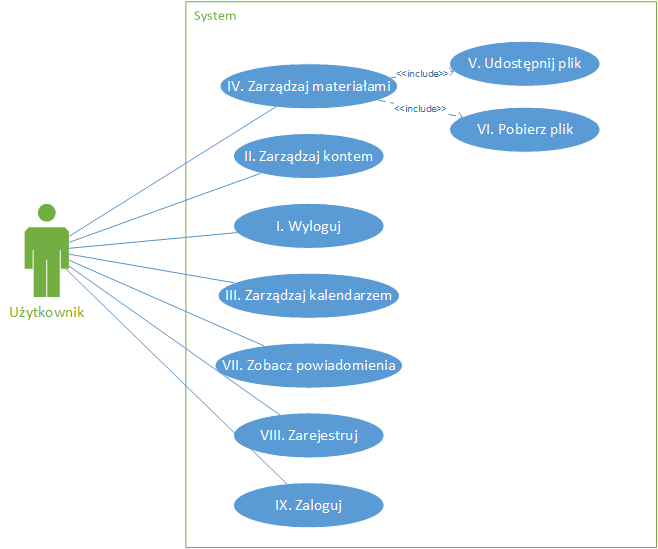
\includegraphics[scale=0.7]{UseCaseUser}
	\caption{\label{fig:caption_01}Diagram przypadków użycia dla użytkownika}
\end{figure}
W poniższym diagramie pominięto przypadki użycia, które posiada zwykły użytkownik, lecz nie należy zapominać, że administrator również je posiada.
\begin{figure}[h]
	\centering
	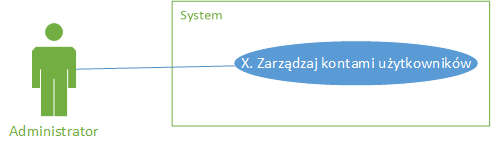
\includegraphics[scale=0.7]{UseCaseAdmin}
	\caption{\label{fig:caption_01}Diagram przypadków użycia dla administratora}
\end{figure}

Scenariusze przypadków użycia:
\begin{table}[h]
\centering
\caption{Wyloguj}
\label{wyloguj}
\begin{tabular}{|p{7cm}|p{7cm}|}
  \hline 
  \textbf{Aktorzy:} & Użytkownik, Administrator\\
  \hline
  \textbf{Zakres:} & System \\
	\hline
  \textbf{Poziom:} & Sytemowowy \\
	\hline
  \textbf{Udziałowcy i ich cele: } & Użytkownik chce się wylogować. \\
	\hline
  \textbf{Zdarzenie wyzwalające } & Użytkownik wciska przycisk “Wyloguj”. \\
	\hline
  \textbf{Warunki wstępne: } & Użytkownik jest zalogowany.
 \\
	\hline
  \textbf{Warunki końcowe dla sukcesu:} & Użytkownik jest wylogowany.
 \\
	\hline
  \textbf{Warunki końcowe dla niepowodzenia:} & Użytkownik jest zalogowany. \\
  \hline
\end{tabular} 
\end{table}
\newpage
\textbf{Scenariusz główny:} \\
1. Użytkownik wciska przycisk wyloguj widoczny w prawym górnym rogu strony. \\
2. Pojawia się okno z napisem: “Czy na pewno chcesz się wylogować?” \\
3. Użytkownik wciska przycisk “tak”. \\
4. Użytkownik jest wylogowany i przekierowany na stronę główną systemu. \\
\textbf{Scenariusz alternatywany: \\
} 
3.a. Użytkownik wciska “nie”. \\
3.a.1. Okno z napisem znika, użytkownik dalej jest zalogowany. \\

\begin{table}[h]
\centering
\caption{Zarządzaj kontem}
\label{zarzadzajkontem}
\begin{tabular}{|p{7cm}|p{7cm}|}
  \hline 
  \textbf{Aktorzy:} & Użytkownik, Administrator\\
  \hline
  \textbf{Zakres:} & System \\
	\hline
  \textbf{Poziom:} & Sytemowowy \\
	\hline
  \textbf{Udziałowcy i ich cele: } & Użytkownik chce zmienić login lub hasło. \\
	\hline
  \textbf{Zdarzenie wyzwalające } & Użytkownik wciska przycisk “Zarządzaj kontem”. \\
	\hline
  \textbf{Warunki wstępne: } & Użytkownik jest zalogowany.\\
	\hline
  \textbf{Warunki końcowe dla sukcesu:} & Login lub hasło użytkownika są zmienione.\\
	\hline
  \textbf{Warunki końcowe dla niepowodzenia:} & Login lub hasło użytkownika nie są zmienione. \\
  \hline
\end{tabular} 
\end{table}

\section{Model systemu}
nad tym tytulem pomyslec!\newline
\subsection{Architektutra systemu}
- najpierw napisac ze soa\newline
- zastanowic sie czy tutaj opis soa czy we wstepie, ale chyba we wstepie, tutaj jedynie można wspomiec ze wczesniej opisany w punkcie X.x.\newline
- Diagram \newline
- byc moze opis

\subsection{Model bazy danych}
- tutaj jakis ladny wstep.\newline
- MODEL ERD - ostateczny \newline

\subsection{Model klas}
- rowniez jakis ladny wstep \newline
- No i diagram klas tutaj ładnie sklepać trzeba będzie \newline

\subsection{Diagramy sekwencji}
- Wstep, ze to wynika z diagramu klas, cos ładnego o diagramach sekwencji - tutaj moze sie wykładami szweda posłużyć \newline
- No i wklepac diagramy sekwencji - moze nie bedzie tak zle jak już beda diagramy klas \newline
\section {Projekt interfejsu?}
Nad tym sie zastanowic czy to robic czy dac dupie siana


\chapter{Projekt architektury systemu}
\label{cha:projektSystemu}
W tym rozdziale omówiona zostanie architektura implementowanego systemu. W pierwszym podrozdziale znajduje się ogólny opis używanej archikterktury, w następnym model bazy danych, a w ostatnim model klas.
\section{Opis architektutry}
Implementowany projekt jest oparty na architekturze SOA (wyjaśnionej w podrozdziale \ref{sec:soa}), która została wybrana przede wszystkim ze względu na podział aplikacji na niezależne od siebie moduły. Dzięki modularności w łatwy sposób można dodawać nowe funkcjonalności do projektu poprzez wstawianie kolejnych usług. Oprócz opisanej wcześniej architektury do implementacji projektu został użyty wzorzec projektowy MVC (\textit{ang. Model View Controller}), który jak sama nazwa wskazuje odpowiada za podzielenie aplikacji na trzy częśći:
\begin{itemize}
	\item Model - część odpowiedzialna za zarządzanie danymi czyli za połączenie z bazą danych,
	\item View - widok odpowiada za interakcję użytkownika z systemem czyli graficzny interfejs użytkownika,
	\item Controller - kontroler oddziałuje pomiędzy modelem a widokiem i kontroluje przepływ danych pomiędzy nimi. \cite{MVC01}
\end{itemize}

Opisywaną architekturę przedstawia poniższy model komponentów:
\begin{figure}[H]
\centering
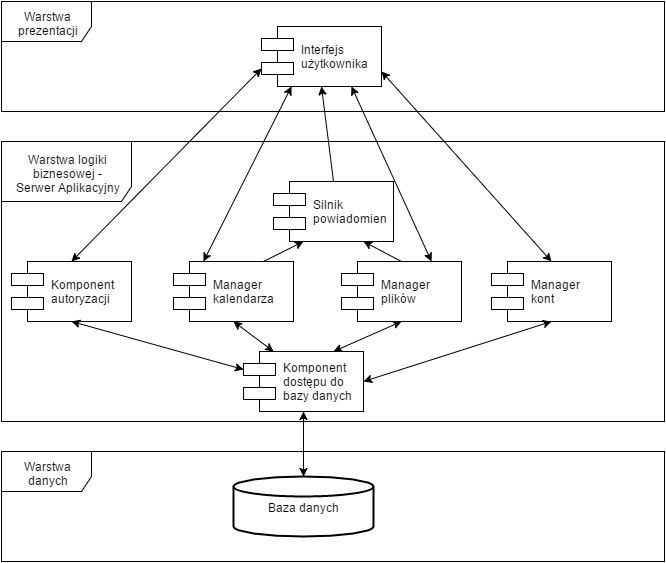
\includegraphics[scale=0.5]{ArchitekturaSystemu}
\caption{\label{fig:diag_01}Diagram komponentów}
\end{figure}
Gdzie każdy z komponentów zostanie opisany dokładnie w rozdziale implementacyjnym.

\section{Model bazy danych}
\label{sec:bd}
Baza danych składa się z sześciu tabel:
\begin{itemize}
	\item User - odpowiedzialna za przechowywanie danych o użytkownikach,
	\item Role - Wyznaczająca rolę użytkownika: \textit{user} lub \textit{admin}, dzięki którym można rozróżnić uprawnienia,
	\item File - Reprezentuje plik,
	\item Calendar - odpowiedzialny za przechowywanie kalendarza użytkownika,
	\item Event - prezentuje wydarzenie,
	\item Shared\_File - dzięki tej tabeli użytkownik może dawać dostęp do swojego pliku innym użytkownikom.
\end{itemize}
Model bazy danych przedstawiony jest poniżej na diagramie ERD:
\begin{figure}[H]
\centering
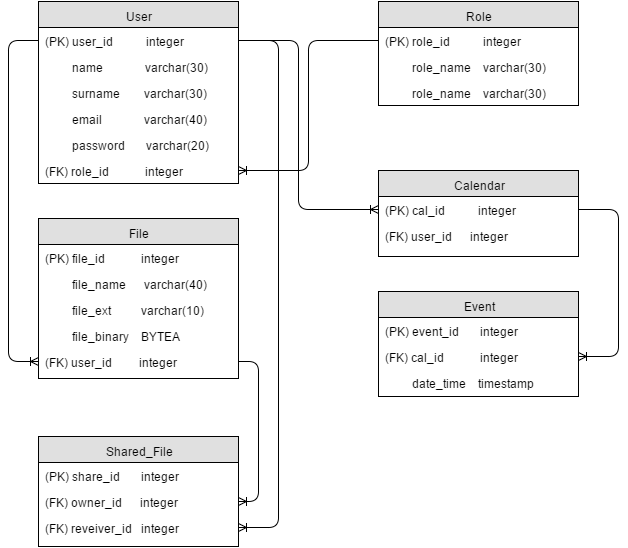
\includegraphics[scale=0.5]{ERD}
\caption{\label{fig:diag_02}Diagram ERD}
\end{figure}

\section{Model klas}
Model klas w postaci diagramu UML reprezentujący tabele z bazy danych:
\begin{figure}[H]
\centering
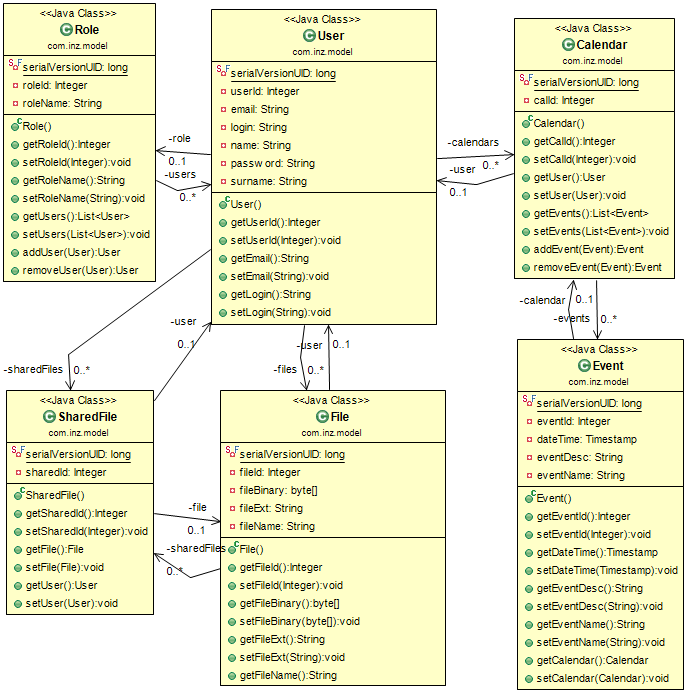
\includegraphics[scale=0.5]{ENTITIES}
\caption{\label{fig:uml_01}Diagram Klas Encji}
\end{figure}
Za połączenie z bazą danych odpowiada wzorzec projektowy DAO (omówiony w \ref{subsec:ejb}), który przedstawiony jest na poniższym diagramie.
\begin{figure}[H]
\centering
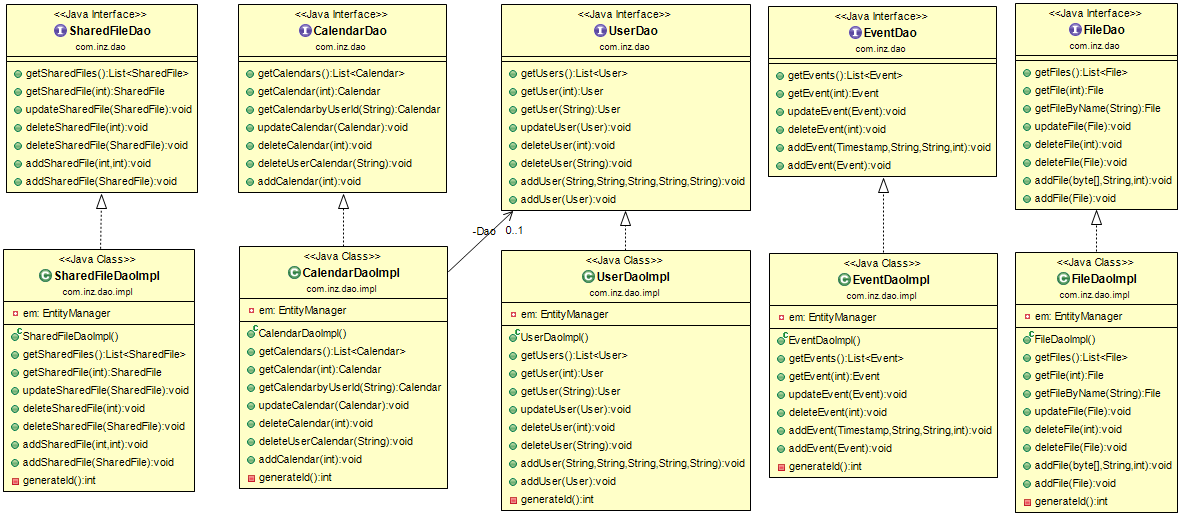
\includegraphics[scale=0.5,angle=90,origin=c]{DAO_UML}
\caption{\label{fig:uml_02}Diagram Klas DAO}
\end{figure}
\chapter{Implementacja}
\label{cha:implementacja}
Rozdział ten opisuje najważniejsze szczegóły implementacyjne projektu. W pierwszym podrozdziale znajduje się krótki opis narzędzi użytych do implementacji oraz sposób w jaki ich użyto. W drugim znajduje się opis podprojektów, a w trzecim metody zabezpieczeń systemu.
\section{Użyte narzędzia}
Aplikacja została zaimplementowana w środowisku programowania \textbf{Eclipse IDE for Java EE Developers}, ponieważ posiada wszystkie niezbędne narzędzia do tworzenia aplikacji JEE. Innym plusem użytego środowiska jest także dodatkowy plugin JBossTools odpowiadający za zarządzanie serwerem aplikacyjnym JBoss.

Dodatkowym bardzo przydatnym narzędziem użytym do implementacji projektu jest \textbf{Apache Maven}, który jest odpowiedzialny za budowanie aplikacji. Tworzenie aplikacji przy użyciu narzędzia maven opiera się na pliku pom.xml (POM – ang. Project Object Model). Jest on miejscem, w którym znajdują się wszystkie najważniejsze informację definiujące projekt, jego strukturę, to w jaki sposób będzie budowany oraz zależności \cite{MV01}. Dużą zaletą Mavena jest łątwy sposób dodawania potrzebnych bibliotek do projektu, co odbywa się za pomocą przyłączania kolejnych zależności do pliku pom.xml, które są automatycznie ściągane z repozytorium mavena. Przykład dodania biblioteki JSF w projekcie:
\begin{lstlisting}
      <dependency>
         <groupId>org.jboss.spec.javax.faces</groupId>
         <artifactId>jboss-jsf-api_2.1_spec</artifactId>
         <scope>provided</scope>
      </dependency>
\end{lstlisting}
Maven posiada archetypy czyli dodatkowe narzędzie do generowania szablonów projektów. Przy tworzeniu opisywanej aplikacji skorzystano z tej właśnie funkcjonalności. Szablon tworzy się za pomocą wywołania komendy:
\begin{lstlisting}
mvn archetype:generate 
\end{lstlisting}
Następnie z pośród tysięcy dostępnych szablonów trzeba wybrać ten, który nas interesuje. W przypadku tego projektu jest to archetyp który buduje szablon aplikacjii JavaEE kompatybilny z serwerem aplikacyjnym JBoss AS 7.1:
\begin{lstlisting}[breaklines=true]
remote -> org.jboss.spec.archetypes:jboss-javaee6-webapp-ear-archetype (An archetype that generates a starter Java EE 6 webapp project for JBoss AS 7.1 (by default) or EAP 6 (if the "enterprise" property is true). The project is an EAR, with an EJB-JAR and WAR)
\end{lstlisting}

Po wybraniu archetypu następuje definicja nazwy projektu oraz nazwy domyślnego pakietu. Wybrany pakiet dzieli projekt na trzy podprojekty: 
\begin{itemize}
	\item EJB - Odpowiedzialny za połączenie z bazą danych. Tutaj znajdują się klasy reprezentujące tabele w bazie danych oraz klasy Bean, które są odpowiedzialne za pobieranie i wstawianie danych z bazy. Podprojekt EJB eksportowany jest w postaci plików JAR (ang. Java archive),
	\item WEB - W tym podprojekcie znajdują się wszystkie strony html tworzące interfejs użytkownika, oraz klasy Managed Bean, które są odpowiedzialne za połączenie ze stronami html. Podczas budowy aplikacji podprojekt WEB zapisywany jest jako WAR (ang. Web archiwe),
	\item EAR - Aplikacja eksportowana jest w postaci plików EAR (enterprise archiwe), które zawierają wszystkie podprojekty implementowanej aplikacji \cite{ECL01}.
%	http://help.eclipse.org/mars/index.jsp?topic=%2Forg.eclipse.jst.j2ee.doc.user%2Ftopics%2Fcjearproj.html).
\end{itemize}
Zbudowany projekt EAR jest lokowany na serwerze aplikacyjnym JBoss.\newline

\section{Oprogramowanie}
Projekt jak to zostało opisane w poprzednim podrozdziale jest podzielony na trzy podprojekty, z których implementacja znajduje się tylko w częściach WEB i EJB. W tym podrozdziale przybliżona zostanie ich zawartość.
\subsection{EJB}
\label{subsec:ejb}
W opisywanym projekcie znajdują się klasy, które zostały wygenerowane dzięki narzędziu JPA Tools (ang. Java Persistance API) z tabel bazy danych opisanych w punkcie \ref{sec:bd}. Przykładowa wygenerowana klasa reprezentująca użytkownika:
\begin{lstlisting}
package com.inz.model;

import java.io.Serializable;
import javax.persistence.*;
import java.util.List;

/**
 * The persistent class for the users database table.
 * 
 */
@Entity
@Table(name="users")
@NamedQueries({
	@NamedQuery(name="user.findAll", query="SELECT u FROM User u"),
	@NamedQuery(name="user.byId", query="select u from User as u where u.userId=:userId"),
	@NamedQuery(name="user.byLogin", query="select u from User as u where u.login=:login"),
})
public class User implements Serializable {
	private static final long serialVersionUID = 1L;

	@Id
	@Column(name="user_id", columnDefinition = "serial")
	private Integer userId;
	private String email;
	private String login;
	private String name;
	private String password;
	private String surname;

	//bi-directional many-to-one association to Calendar
	@OneToMany(mappedBy="user")
	private List<Calendar> calendars;

	//bi-directional many-to-one association to File
	@OneToMany(mappedBy="user")
	private List<File> files;

	//bi-directional many-to-one association to SharedFile
	@OneToMany(mappedBy="user")
	private List<SharedFile> sharedFiles;

	//bi-directional many-to-one association to Role
	@ManyToOne
	@JoinColumn(name="role_id")
	private Role role;

	public User() {
	}

	/* Metody get i set dla wszystkich atrubutów */
}
\end{lstlisting}

W powyższym przykłądzie ominięte zostały metody get i set odpowiadające za pobieranie i ustawianie atrybutów klasy. Właściwości tabeli w wygenerowanej klasie są zachowane dzięki adnotacjom (@Adnotacja), gdzie @Id definiuje klucz główny tabeli, @OneToMany i @ManyToOne relacje zachodzące między tabelami i @Column podający dodatkowe właściwości kolumny, które nie mogą być przedstawione przy pomocy zmiennej w języku Java. Ponadto ponad definicją klasy znajdują się adnotacje @Entity, która oznacza klasę jako reprezentującą tabelę z bazy danych, @Table pozwalająca ustawić nazwę tabeli do której się odwołuje oraz @NamedQueries, która pozwala na zdefiniowanie w prosty sposób zapytań do bazy danych. Dzięki frameworkowi JPA i wygenerowanym przez niego klasom nie trzeba się odwoływać do tabel z bazy, lecz do powstałych klas.

Aby ułatwić innym komponentom dostęp do bazy danych skorzystano z wzorca projektowego DAO (ang. Data Access Object), który tworzy jednolity interfejs odpowiedzialny za połączenie z bazą danych. DAO sprawia, że warstwa odpowiadająca za logike aplikacji nie musi znać szczegółów implementacyjnych udostępnionego interfejsu co uniezależna tą warstwę od sposobu dostępu do bazy danych. Poniżej zostanie przedstawiony przykładowy interfejs i jego implementacja odpowiedzialne za zarządzanie tabelą użytkownika.\\
Interfejs:
\begin{lstlisting}[breaklines=true]
package com.inz.dao;

import java.util.List;
import com.inz.model.User;

public interface UserDao {
	List<User> getUsers();
	User getUser(int id);
	User getUser(String login);
	void updateUser(User user);
	void deleteUser(int id);
	void deleteUser(String login);
	void addUser(String login, String name, String surname, String email, String password);
	void addUser(User user);
}
\end{lstlisting}
Implementacja:
\begin{lstlisting}[breaklines=true]
package com.inz.dao.impl;

import java.util.LinkedList;
import java.util.List;

import javax.ejb.Local;
import javax.ejb.Stateless;
import javax.ejb.TransactionAttribute;
import javax.ejb.TransactionAttributeType;
import javax.persistence.EntityManager;
import javax.persistence.PersistenceContext;

import com.inz.dao.UserDao;
import com.inz.model.User;

@Stateless
@Local(UserDao.class)
@TransactionAttribute(TransactionAttributeType.REQUIRED)
public class UserDaoImpl implements UserDao {

	@PersistenceContext(name="primary")
	private EntityManager em;
	
	@Override
	public List<User> getUsers() {
		return em.createNamedQuery("user.findAll").getResultList();
	}

	@Override
	public User getUser(int id) {
		return (User) em.createNamedQuery("user.byId")
			.setParameter("userId", id).getSingleResult();
	}

	@Override
	public User getUser(String login) {
		return (User) em.createNamedQuery("user.byLogin")
			.setParameter("login", login).getSingleResult();
	}

	@Override
	public void updateUser(User user) {
		em.merge(user);
	}

	@Override
	public void deleteUser(int id) {
		User u = getUser(id);
		em.remove(u);
	}

	@Override
	public void deleteUser(String login) {
		User u = getUser(login);
		em.remove(u);
	}

	@Override
	public void addUser(String login, String name, String surname, String email,
			String password) {
		User u = new User();
		u.setLogin(login);
		u.setName(name);
		u.setSurname(surname);
		u.setEmail(email);
		u.setPassword(password);
		u.setUserId(generateId());
		em.persist(u);
	}

	@Override
	public void addUser(User user) {
		if(user.getUserId().equals(null)){
			user.setUserId(generateId());
		}
		em.persist(user);
	}
	
	private int generateId(){
		List<User> users = getUsers();
		int id=0;
		List<Integer> ints = new LinkedList<Integer>();
		for(User usr:users){
			ints.add(usr.getUserId());
		}
		int i=1;
		while(true){
			if(ints.contains(i)) i++;
			else{
				id=i;
				break;
			}
		}
		return id;
	}
}
\end{lstlisting}

Najważniejszą zmienną odpowiedzialną za wykonywanie operacji na bazie danych jest instancja klasy EntityManager, która jest "wstrzyknięta" do klasy za pomocą adnotacji @PersistenceContext. Adnotacja @Stateless oznacza, że wstrzykniwany Bean (komponent wielokrotnego użytku w różnych miejscach aplikacji) będzie bezstanowy. Komponent ten jak sama nazwa wskazuje nie posiada żadnego stanu więc wszystkie takie komponenty wywoływane przez różnych użytkowników są identyczne. Adnotacja @Local mówi o tym, że implementowany interfejs znajduje się w tym samym środowisku. Adnotacja @TransactionAttribute(TransactionAttributeType.REQUIRED) wymusza na każdej metodzie, aby była wykonana w ramach tranzakcji już działającej, a jeżeli żadna nie jest rozpoczęta to musi być utworzona nowa. Stworzony bean wstrzykuje się w następujący sposób:
\begin{lstlisting}
@EJB private UserDao dao;
\end{lstlisting}

\subsection{WEB}
Użytkownik korzysta z aplikacją za pomocą przeglądarki internetowej, więc interfejsem są strony www. W implementowanej aplikacji są to pliki z rozszerzeniem xhtml. Głównym frameworkiem pomocnym przy tworzeniu tego interfejsu jest JSF, który udostępnia dodatkowe tagi pomocne przy tworzeniu stron oraz klasy Managed Bean dzięki którym można się połączyć z tymi stronami.\\
Przykładowy formularz odpowiedzialny za rejestracje nowego użytkownika:
\begin{lstlisting}[breaklines=true]
<?xml version="1.0" encoding="UTF-8" ?>
<!DOCTYPE html PUBLIC "-//W3C//DTD XHTML 1.0 Transitional//EN" "http://www.w3.org/TR/xhtml1/DTD/xhtml1-transitional.dtd">
<html 	xmlns="http://www.w3.org/1999/xhtml" 
		xmlns:h="http://java.sun.com/jsf/html"
		xmlns:f="http://java.sun.com/jsf/core"> 
<h:head>
<meta http-equiv="Content-Type" content="text/html; charset=UTF-8" />
<title>Rejestracja</title>
</h:head> 
<h:body>  
	Zarejestruj się: 
	<h:form>
	<br />
	   Login: <h:inputText id="login" value="#{userMan.login}" 
	   			required="true"
	   			validator="#{userMan.validateLogin}"
	   			requiredMessage="Pole Login jest wymagane."/> 
	   			<h:message for="login" style="color:red" /> <br />
	   Hasło: <h:inputSecret id="password" value="#{userMan.password}" 
					required="true" 
	   			validatorMessage="Błąd walidacji: Hasło nie może zawierać znaków specjalnych oraz musi mieć długość od 5 do 30 znaków."
	   			requiredMessage="Pole Hasło jest wymagane.">  
	   			<f:validateRegex
					pattern="[A-Za-z0-9]*{5,30}$" />
			    </h:inputSecret>
			    <h:message for="password" style="color:red" /> <br />
		Imię: <h:inputText id="name" value="#{userMan.name}" 
				required="true"  
				requiredMessage="Pole Imię jest wymagane."/> 
				<h:message for="name" style="color:red" /> <br />
	Nazwisko: <h:inputText id="surname" value="#{userMan.surname}" 
				required="true" 
				requiredMessage="Pole Nazwisko jest wymagane."/> 
				<h:message for="surname" style="color:red" /> <br />
	   Email: <h:inputText id="email" value="#{userMan.email}" 
				required="true" 
				validatorMessage="Błąd walidacji: Email musi być postaci użytkownik@domena."
				requiredMessage="Pole Email jest wymagane."> 
				<f:validateRegex
					pattern="^[_A-Za-z0-9-\+]+(\.[_A-Za-z0-9-]+)*@[A-Za-z0-9-]+(\.[A-Za-z0-9]+)*(\.[A-Za-z]{2,})$" />
			  </h:inputText>
			  <h:message for="email" style="color:red" /> <br />
		<h:commandButton value="Dodaj mnie" action="#{userMan.addUser()}" />
	</h:form>
</h:body>
</html>
\end{lstlisting}
Klasa Managed Bean odpowiedzialna za obsługę powyższego formularza:
\begin{lstlisting}[breaklines=true]
package com.inz.jsf;

import java.util.List;
import javax.ejb.EJB;
import javax.faces.application.FacesMessage;
import javax.faces.bean.ManagedBean;
import javax.faces.bean.SessionScoped;
import javax.faces.component.UIComponent;
import javax.faces.context.FacesContext;
import javax.faces.validator.ValidatorException;
import com.inz.dao.UserDao;
import com.inz.model.User;

@ManagedBean(name = "userMan", eager = true)
@SessionScoped
public class UserManager {
	@EJB private UserDao dao;
	private String login;
	private String name;
	private String surname;
	private String password;
	private String email;
	
	public void ManagedBean(){};
	
/* Metody get i set */

	public String addUser(){
		dao.addUser(login, name, surname, email, password);
		return "index";
	}
	
	public void validateLogin(FacesContext context, UIComponent component, Object value) throws ValidatorException {
		  String login = (String) value;
		  String message = "Błąd walidacji: ";
		  boolean err = false;
		  if ( login.length() > 30 || login.length() < 5 ) {
			  message=message+"Login musi mieś długość od 5 do 30 znaków.";
			  err=true;
		  } else if(validateLoginHelper(login)){
			  message=message+"Użytkownik o podanym loginie znajduje się już w bazie danych.";
			  err=true;
		  }  
		  if(err){
			  FacesMessage msg = new FacesMessage(message);
		      throw new ValidatorException(msg);
		  }
		}
	
	private boolean validateLoginHelper(String login){
		List<User> users = dao.getUsers();
		for(User u:users){
			if(u.getLogin().equals(login)) return true;
		}
		return false;
	}
}
\end{lstlisting}

ManagedBean to klasa z frameworku JSF, która jest dostępna ze stron używających tagów JSF. Definiowana jest za pomocą adnotacji @ManagedBean. Adnotacja @SessionScoped definiuje, że Bean żyje tak długo jak sesja HTTP. 

Aby użytkownik nie mógł wprowadzać nieprawidłowych danych przy tworzeniu formularza zastosowano mechanizm walidacji wprowadzanych danych. Użytkownik nie może zostawić pola nieuzupełnionego (required="true"), a ponadto do pola login, hasło i email są sprawdzane pod względem wprowadzanego tekstu. W polach email i hasło sprawdzany jest warunek długości oraz treści wprowadzanego tekstu za pomocą wyrażenia regularnego na stronie JSF (f:validateRegex pattern="warunek"). Pole login walidowane jest za pomocą MangedBeana pod względem długości tekstu (od 5 do 30 znaków) oraz unikalności loginu w systemie. Jeżeli któryś z wyżej opisanych warunków nie zostanie spełniony to po prawej stronie pola pojawi się odpowiedni komunikat w kolorze czerwonym.

\section{Zabezpieczenia}
Wszystkie usługi będą udostępniane tylko zalogowanym użytkownikom. Możliwość zarządzania plikami oraz kalendarzem wszystkich użytkowników posiada tylko administrator, co jest autoryzowane za pomocą bazy danych oraz podsystemu bezpieczeństwa serwera aplikacyjnego JBoss. 

W celu stworzenia logowania do systemu skorzystano z pomocy modułu logowania \textit{Database} dostarczanego przez serwer aplikacyjny JBoss. Aby zrealizować autoryzację w pierwszej kolejności trzeba dodać odpowiednie elementy do pliku konfiguracyjnego serwera JBoss (standalone.xml):
\begin{lstlisting}[breaklines=true]
<security-domain name="postgresql-domain" cache-type="default">
	<authentication>
		<login-module code="Database" flag="required">
			<module-option name="dsJndiName" value="java:jboss/datasources/StudentServisDataSource"/>
			<module-option name="principalsQuery" value="select password from users where login=?"/>
			<module-option name="rolesQuery" value="select role_name, 'Roles' as Roles from role r join users u on (r.role_id=u.role_id) where u.login=?"/>
		</login-module>
	</authentication>
</security-domain>
\end{lstlisting}
Powyższy wpis definiuje moduł logowania korzystający z weryfikacji za pomocą bazy danych zdefiniowanej w źródle danych \textit{StudentServisDataSource}. Następnie przygotowany jest specjalny formularz logowania, po czym w pliku xml między znacznikami <security-constraint> definiowane są strony, do których dostęp ma tylko zalogowany użytkownik. Dodatkowo w pliku web.xml definiowane są strony logowania do których niezalogowany użytkownik jest przekierowywany gdy chce uzyskać dostęp do stron objętych ochroną:
\begin{lstlisting}[breaklines=true]
		<form-login-config>
			<form-login-page>/login.xhtml</form-login-page>
			<form-error-page>/login_error.xhtml</form-error-page>
		</form-login-config>
\end{lstlisting}
Aby przydzielić niektóre funkcje systemu tylko administratorowi nad ManagedBeanem wstawiane są następujące adnotacje:
\begin{lstlisting}[breaklines=true]
@RolesAllowed("admin")
@SecurityDomain("postgresql-domain") 
\end{lstlisting} 
Gdzie adnotacja @SecurityDomain definiuje baze danych na podstawie której użytkownik rola użytkownika jest weryfikowana.

\chapter{Podsumowanie}
\label{cha:podsumowanie}
W podsumowaniu pracy należy zebrać wnioski z jej realizacji. Odpowiedzieć na pytania: czy
cel pracy został osiągnięty i w jakim stopniu. Co inaczej byłoby realizowane, gdyby autor od
nowa zaczął tę pracę? Można tu podać trochę ciekawostek z jej realizacji. Kto i jaki pożytek
może mieć z tej pracy? Czy warto kontynuować tą pracę i w jaki sposób? Jakie nowe
problemy zostały zidentyfikowane i które z nich mogę być przedmiotem kolejnych prac
dyplomowych? Podsumowanie nie ma na celu wykazywać, że stworzony produkt jest idealny
i bezbłędny, lecz to, że autor jest rzetelnym i kompetentnym projektantem i analitykiem. Do
błędów popełnionych w pracy należy się uczciwie przyznać. \newline
Tutaj bez podrozdzialow.


\printbibliography



\end{document}
